\begin{minipage}{0.45\linewidth}
  % Reduced vertical spacing
\setlength{\abovedisplayskip}{0pt}
\setlength{\belowdisplayskip}{0pt}
\begin{enumerate}
\item left/right associativity:
  \[
    S \rightarrow S - S \Rightarrow\left\{
      \begin{array}{l}
        S \rightarrow S - \mathsf{int} \\
        S \rightarrow \mathsf{int} - S
      \end{array}
       \right.
  \]
\item higher precedence: the \(V_{n}\) \textbf{closer} to \(V_{t}\) or use \verb|()|
  \begin{itemize}[leftmargin=1.5em]
    \item[$P_{1}$] \(S \rightarrow S + T \gor T\)
    \item[] ``+'' can't break \(T\)
    \item[$P_{2}$] \(T \rightarrow T * \mathsf{int} \gor \mathsf{int}\)
    \item[] positioned lower than \(P_{1}\)
    \item \(P_{2}\) has \textbf{higher} priority: always expand \(T\) first
    \end{itemize}
\item Controlling \(\epsilon\) (only derived from \(S\)):
  \[
    S \rightarrow \epsilon \gor (S) \gor SS \Rightarrow\left\{
        \begin{array}{l}
          S \rightarrow \epsilon \gor T\\
          T \rightarrow TU \gor U\\
          U \rightarrow () \gor U \rightarrow (T)
        \end{array}
      \right.
  \]
\end{enumerate}
\end{minipage}
\begin{minipage}[t]{0.45\linewidth}
  \centering
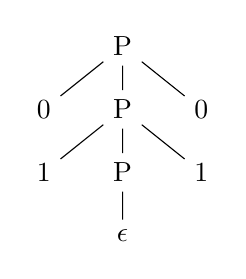
\begin{tikzpicture}[level distance=8mm,level/.style={sibling distance=10mm}]
  \node {P}
  child {node {0}}
  child {
    node {P}
    child {node {1}}
    child {
      node {P}
      child {node {\(\epsilon\)}}
    }
    child {node {1}}
  }
  child {node {0}};
\end{tikzpicture}\\
\emph{un}ambiguous grammar: \textbf{unique} parse tree of given string.  Concatenate leaves (\(V_{t}/\epsilon\)) of a parse tree \textbf{anti-clockwise} and get the \textbf{yield} of the parse tree: \textbf{0110}
\end{minipage}
